\chapter{Rancangan}
\label{chap:rancangan}
Bab ini menjelaskan perancangan aplikasi, termasuk algoritma-algoritma untuk mengolah \textit{Google StreetView API}, \textit{Google Directions API}, serta modifikasi yang dilakukan pada aplikasi HelloVR untuk membangun aplikasi \textit{jogging} virtual. 

\section{Rancangan Antarmuka}
Aplikasi yang akan dibangun terdiri atas dua \textit{activity}, yaitu \textit{activity} utama dan \textit{activity} VR.

\subsection{\textit{Activity} Utama}
\label{subs:main-page}
\textit{Activity} utama adalah \textit{activity} yang ditampilkan pertama kali saat pengguna membuka aplikasi dengan \textit{portrait layout}. Fungsi \textit{activity} ini adalah menerima masukan pengguna, yaitu lokasi asal dan lokasi tujuan saat berlari, serta memicu \textit{activity} kedua, yaitu \textit{activity} VR. Ada tiga komponen utama dari \textit{activity} ini, yaitu dua buah \textit{textbox} dan sebuah tombol. Satu \textit{textbox} adalah \textit{textbox} "\textit{origin}", dan \textit{textbox} yang lain adalah \textit{textbox} "\textit{destination}". Gambar \ref{fig:main-page} menggambarkan tampilan \textit{activity} utama.  

\begin{figure}[!hp]
  \centering
    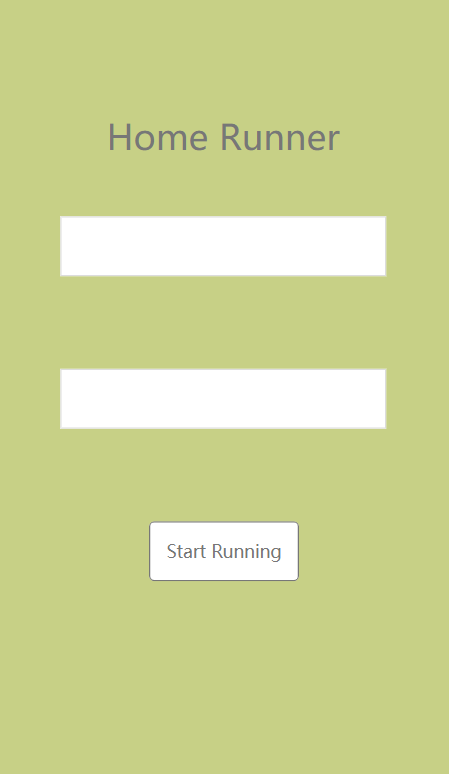
\includegraphics[scale=0.7]{Gambar/mockup-main-activity.png}
    \caption{Rancangan \textit{Activity} utama aplikasi}\label{fig:main-page}
\end{figure}


\subsubsection{\textit{Textbox Origin}} 
\textit{Textbox} adalah komponen pada antarmuka yang menerima masukan pengguna yang berupa tulisan atau \textit{string}. \textit{Textbox} "\textit{origin}" akan menerima masukan pengguna yang merupakan lokasi asal dari rute lari.

\subsubsection{\textit{Textbox Destination}}
\textit{Textbox Destination} adalah \textit{textbox} kedua dan berada di bawah \textit{textbox origin}  akan menerima masukan berupa lokasi tujuan dari rute lari yang dimasukkan pengguna.   

\subsubsection{Tombol ``\textit{Start Running}''}
Tombol "\textit{Start Running}" adalah tombol yang akan memicu \textit{activity} VR yang sesuai dengan informasi dari dua \textit{textbox} di atas ketika ditekan. Tombol ini berada di bawah \textit{destination textbox}.

\subsection{\textit{Activity} VR}
\textit{Activity} VR adalah \textit{activity} yang menampilkan pemandangan VR secara VR ketika berlari. Untuk memunculkan \textit{activity} ini, pengguna harus menekan tombol dari \textit{activity} utama (dijelaskan pada Subbab \ref{subs:main-page}) terlebih dahulu. Karena posisi gawai masih dalam keadaan \textit{portrait}, ada satu \textit{activity} terlebih dahulu yang muncul seperti di Gambar \ref{fig:cardboard-page}. 

\textit{Activity} ini dimunculkan ketika mengakses \textit{Google Cardboard}. Untuk menuju ke \textit{activity} VR, pengguna harus memutar gawai sehingga gawai berada dalam posisi \textit{landscape}. Setelah gawai berada dalam posisi \textit{landscape}, \textit{activity} VR akan dimunculkan seperti yang ditunjukkan pada Gambar \ref{fig:vr-page}.

\begin{figure}[h]
	\centering
		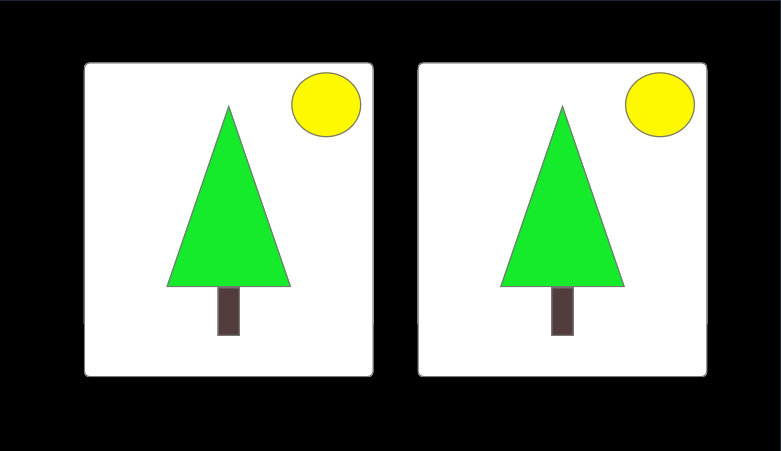
\includegraphics[scale=0.7]{Gambar/mockup-vr-page.png}
	\caption{Rancangan \textit{Activity} VR}
	\label{fig:vr-page}
\end{figure}

Pada tampilan VR tersebut, gambar akan berubah-ubah sesuai dengan langkah kaki pengguna. Perubahan tersebut akan terjadi ketika mencapai pengguna mencapai jarak 100 meter. Jika pengguna sudah mencapai tujuan sesuai dengan jarak yang ditempuh, \textit{activity} VR akan berhenti mengubah gambar.     

\section{Rancangan Program}
Subbab ini akan menjelaskan rancangan  program, mulai dari rancangan kelas dan algoritma-algoritma yang digunakan pada \textit{method-method} yang penting. 

\subsection{Rancangan Kelas}
Rancangan kelas dari aplikasi akan menggunakan seluruh bagian pada aplikasi HelloVR dan beberapa tambahan kelas. Gambar \ref{fig:class-diagram} menunjukkan atribut-atribut dan \textit{method-method} dari masing-masing kelas, serta hubungan antara satu kelas dan kelas-kelas lain. 

\begin{figure}[h]
	\centering
		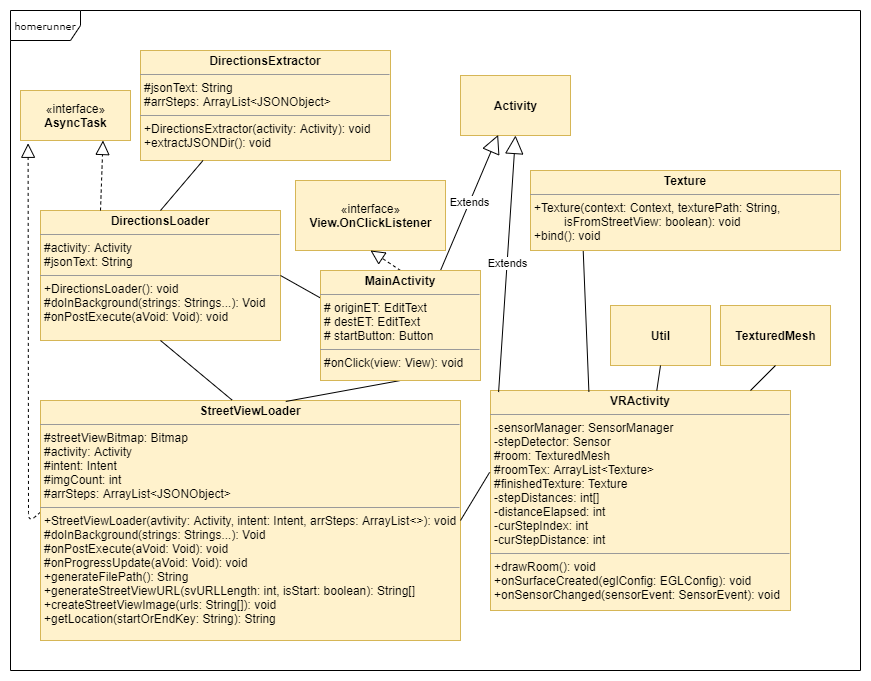
\includegraphics[scale=0.6]{Gambar/class-diagram.png}
	\caption{Diagram \textit{class} dari Aplikasi}
	\label{fig:class-diagram}
\end{figure}

Beberapa kelas di Gambar \ref{fig:class-diagram} tidak memiliki deskripsi lebih karena berasal dari \textit{library} Java ataupun \textit{Google VR SDK}. Kelas-kelas yang ditambahkan adalah:

%Lengkapi penjelasan
\begin{enumerate}
	\item \texttt{MainActivity}
	
	Kelas yang mengelola \textit{activity} utama. Atribut yang dimiliki kelas ini:
	
	\begin{itemize}
		\item \texttt{protected EditText originET}
		
		Bagian dari antarmuka yang dapat menerima masukan lokasi asal dari rute lari.
		\item \texttt{protected EditText destET}
		
		Bagian antarmuka yang dapat menerima masukan lokasi tujuan dari rute lari.
		\item \texttt{protected Button startButton}
		
		Tombol yang digunakan untuk memuat rute perjalanan dan gambar pemandangan, serta memicu \textit{activity} VR.
	\end{itemize}
	
	\textit{Method-method} yang dimiliki kelas ini adalah:
	
	\begin{itemize}
		\item \texttt{protected void onClick(View view)}
		
		\textit{Method} yang dijalankan ketika komponen yang sudah dipasangkan \texttt{onClickListener} ditekan. 
		
	\end{itemize}
	\item \texttt{VRActivity}
	
	\textit{Class} yang mengelola activity VR. Atribut-atribut yang dimiliki \textit{class} ini adalah:
	
	\begin{itemize}
		\item \texttt{private SensorManager sensorManager}
		
		Atribut yang mengatur sensor dari gawai Android.
		\item \texttt{private Sensor stepDetector}
		
		Sensor pendeteksi langkah kaki.
		\item \texttt{protected TexturedMesh room}
		
		Bangun ruang VR yang sudah dipasangkan dengan objek \textit{Texture}.
		\item \texttt{protected ArrayList<Texture> roomTex}
		
		\textit{ArrayList} dari gambar-gambar \textit{StreetView} yang merupakan tekstur dari bangun ruang VR.
		\item \texttt{protected Texture finishedTexture}
		
		Gambar dari tekstur bangun ruang VR yang menandakan perjalanan pengguna sudah selesai.

		\item \texttt{private int[] stepDistances}		
		
		\textit{Array} dari jarak setiap \textit{steps} dari rute lari.	
		\item \texttt{private int distanceElapsed}
		
		Atribut ini menyimpan jarak yang sudah ditempuh pengguna.
		\item \texttt{private int curStepIndex}
		
		Atribut yang menyimpan \textit{index} dari \textit{step} yang sedang ditempuh saat ini.
		\item \texttt{private int curStepDistance}

		Atribut yang menyimpan penjumlahan jarak dari \textit{step} saat ini dan jarak dari setiap \textit{steps} yang sudah ditempuh.		
	\end{itemize}
	
	\textit{Method-method} yang dimiliki \textit{class} ini adalah:
	
		\begin{itemize}
			\item \texttt{public void drawRoom()}
			
			\textit{Method} untuk menggambar ruangan tiga dimensi.
			\item \texttt{public void onSurfaceCreated(EGLConfig eglConfig)}
			
			\textit{Method} yang dipanggil ketika permukaan VR diciptakan. Parameter yang dimiliki \textit{method} ini adalah:
			
			\begin{itemize}
				\item \texttt{EGLConfig eglConfig}
				
			Konfigurasi dari  \textit{OpenGL renderer}. 				
			\end{itemize}
		
		\textit{Method} ini tidak memiliki nilai kembali.
		\item \texttt{public void onSensorChanged(SensorEvent sensorEvent)}
		
		\textit{Method} yang dipanggil ketika sensor \textit{step detector} mendeteksi \textit{event}.	
		\end{itemize}
	
	\item \texttt{StreetViewLoader}
	
	\textit{Class} yang berfungsi untuk memuat gambar \textit{StreetView} dan menyatukan semua gambar itu, membentuk gambar pemandangan yang utuh. Atribut-atribut yang dimiliki \textit{class} ini adalah:
	
	\begin{itemize}
		\item \texttt{protected Bitmap streetViewBitmap}
		
		Atribut yang menampung \textit{Bitmap} dari \textit{StreetView} yang telah diunduh dari \textit{StreetView API}.	
		\item \texttt{protected Activity activity}
		
		\textit{Activity} yang dihubungkan dengan \textit{class} ini  sehingga komunikasi antara objek dua kelas ini dapat terjadi.
		
		\item \texttt{protected Bitmap streetViewBitmap}
		
		Atribut untuk menyimpan \textit{bitmap} dari gambar \textit{StreetView}.
		\item \texttt{protected Activity activity}
		
		Atribut dari \textit{activity} yang memanggil \textit{method} dari \textit{class} ini sehingga data dan nilai yang sudah diperoleh dari \textit{class} ini dapat diserahkan pada \textit{activity} ini. \textit{Method} ini tidak memiliki nilai kembali.
		\item \texttt{protected Intent intent}  
		
		\textit{Intent} dari \textit{activity} yang memicu \textit{activity} untuk dijalankan.
		\item \texttt{protected int imgCount}
		
		Atribut yang menyimpan angka perhitungan setiap kali gambar dimuat dari \textit{StreetView API}.
		\item \texttt{protected ArrayList<JSONObject> arrSteps}
		
		\textit{Arraylist} dari \textit{JSON Object} dengan \textit{key} "\textit{steps}" dari JSON yang diperoleh dari \textit{Directions API}.
	\end{itemize}
	
	\textit{Method-method} yang dimiliki \textit{class} ini adalah:
	
	\begin{itemize}
		\item \texttt{protected doInBackground(Void... aVoid}
		
		\textit{Method} yang memuat dan menyatukan gambar-gambar \textit{StreetView API}, yang dijalankan pada \texttt{AsyncTask} berbeda. 				
		\item \texttt{protected Void onPostExecute(Void aVoid)}
		
		\textit{Method} yang dipanggil setelah \texttt{doInBackground()} selesai dijalankan, untuk memicu \textit{VrActivity}.
		\item \texttt{public String[] generateStreetViewURL(int svUrlLength, boolean isStart)}
		
		\textit{Method} ini akan men-\textit{generate} URL untuk mengakses  \textit{StreetView API}. 
		
		Parameter:
		
		\begin{itemize}
			\item \texttt{int svUrlLength}
			
			Parameter ini menyatakan berapa banyak \textit{string} URL untuk mendapatkan gambar-gambar StreetView.
			\item \texttt{boolean isStart}
			
			Nilai \textit{boolean} yang menandakan apakah \textit{key} dari \textit{JSONObject} \textit{start\_location} atau \textit{end\_location}.
		\end{itemize}
		
		Nilai Kembalian:
	
		\begin{itemize}
			\item \texttt{String[] urlArr}
		
			\textit{Array} dari URL \textit{StreetView API} yang sudah di-\textit{generate}.		
		\end{itemize}
	\end{itemize}		
	
	\item \texttt{DirectionsLoader}
	
	\textit{Class} yang memuat JSON dari rute lari. Atribut-atribut yang dimiliki kelas ini adalah:
	\begin{itemize}
	
		\item \texttt{protected Activity activity}
		
		\textit{Activity} yang diacu agar dapat berhubungan dengan objek dari \textit{class} ini.
	
		\item \texttt{protected String jsonText}
		
		Atribut yang menyimpan \textit{text} yang diperoleh dari \textit{Directions API}.
	\end{itemize}
	
	\textit{Method-method} yang dimiliki \textit{class} ini adalah:
	
	\begin{itemize}
		\item \texttt{protected Void doInBackground(Strings... strings)}
		
		\textit{Method} yang dijalankan di \texttt{AsyncTask} berbeda, yaitu untuk memuat \textit{file} JSON \textit{Directions API}.
		\item \texttt{protected Void onPostExecute(Void aVoid)}
		
		\textit{Method} yang dijalankan setelah \textit{method} \texttt{doInBackgroud()} selesai dijalankan, untuk mem-\textit{parse} JSON lewat objek dari \textit{class} \texttt{DirectionsExtractor} \textit{Directions API}, lalu memanggil menginstansiasi objek dari \textit{class} \texttt{StreetViewLoader}. 
	\end{itemize} 
	
	\item \texttt{DirectionsExtractor}
	
	\textit{Class} yang berfungsi sebagai \textit{parser} JSON yang diperoleh dari \textit{Directions API}. Atribut yang ada pada \textit{class} ini adalah:
	
	\begin{itemize}
		\item \texttt{protected ArrayList<JSONObject> arrSteps}
		
		\textit{ArrayList} dari objek-objek \textit{steps} yang diperoleh dari \textit{Directions API}.
		\item \texttt{protected String jsonText}
		
		\textit{Text} JSON yang diperoleh dari \textit{Directions API}. 
	\end{itemize}
	
	\textit{Method} yang ada pada \textit{class} ini adalah:
	
	\begin{itemize}
		\item \texttt{protected void extractJSONDir()} 
		
		\textit{Method} yang akan mengambil bagian \textit{steps} dari JSON \textit{Directions API}.	
	\end{itemize}
\end{enumerate} 

\subsection{Algoritma-Algoritma yang Digunakan}
Ada beberapa algoritma yang digunakan   untuk melakukan beberapa proses seperti mengolah \textit{Google StreetView API},\textit{Google Directions API}, dan pemanfaatan sensor \textit{step detector}.

\subsubsection{Pemanfaatan \textit{Google Directions API}}
\textit{Directions API} adalah \textit{API} yang menggunakan protokol HTTP/HTTPS dan menghasilkan keluaran dalam bentuk JSON. Untuk memuat JSON berisi rute perjalanan dari asal sampai tujuan, pemanggilan \textit{Directions API} harus dilakukan melalui HTTP/HTTPS.

\begin{algorithm}
	\caption{Algoritma Mengunduh JSON dari \textit{Directions API} dan \textit{Parsing}}
	\label{alg:algoritma-directions-parsing}
	\begin{algorithmic}[1]
	\Function{processJSONDirections}{$originLoc$,$destLoc$}
		\State $dirText \gets getJSONFromDirAPI(originLoc,destLoc)$ 
		
		\State $dirJSON \gets toJSON(dirText)$	
		
		\State $jsonRoute \gets dirJSON.getJSONObject("routes")$
		
		\State $jsonArrLegs \gets jsonRoute.getJSONArray("legs")$

		\State Declare Array $processedJSONObj$		
		
		\For {$elements in jsonArrLegs$}
		\State $jsonLegs \gets element.getJSONObject("legs") $

		\State $jsonArrSteps \gets jsonLegs.getJSONArray("steps")$		
		
		\State Insert all elements from $jsonArrSteps$ to $processedJSONObject$ 
		\EndFor
	\EndFunction  
	\end{algorithmic}
\end{algorithm}

Setelah JSON rute diperoleh, JSON rute lari dapat digunakan dengan membaca atribut dan nilai-nilainya sesuai kebutuhan. Beberapa nilai atribut dalam JSON ini  berupa JSON \textit{object}, ada yang berupa JSON \textit{array}. Karena hal ini,  \textit{parsing} dari JSON ini harus dilakukan sesuai dengan ketentuan tersebut. Algoritma \textit{parsing} dari JSON \textit{Directions} dipaparkan pada \ref{alg:algoritma-directions-parsing}. 

Setelah JSON dari \textit{Directions API} diunduh, \textit{parsing} adalah langkah selanjutnya untuk mengambil informasi yang dibutuhkan. Karena bagian \textit{steps} yang harus diambil, haruslah \textit{value} dari \textit{key legs} harus diperoleh terlebih dahulu. Selanjutnya, \textit{JSON Array} yang merupakan \textit{value} dari \textit{key} \textit{"legs"}, dan objek-objek dari \textit{JSON Array} \textit{steps} itu dapat dimasukkan ke dalam sebuah struktur data seperti \textit{array} agar dapat digunakan.  

\subsubsection{Algoritma Memperoleh dan Mengolah \textit{Google StreetView API}} 
\textit{StreetView API} berfungsi untuk memuat gambar pemandangan dan menggunakan menggunakan HTTP/HTTPS. Karena satu kali pemanggilan hanya menghasilkan gambar dari satu \textit{heading} atau arah, beberapa gambar dari beberapa arah pandangan haruslah diunduh terlebih dahulu. Setelah semua gambar itu terunduh, semua gambar itu disatukan, menjadi satu gambar untuk menjadi tekstur bangun ruang silinder. Setelah gambar-gambar itu sudah disatukan, gambar tersebut harus disimpan di dalam \textit{file}.

Karena pemandang yang harus diunduh adalah gambar dari lokasi asal dan tujuan dari pengguna untuk membentuk perjalanan lari dari pengguna, gambar-gambar dari lokasi asal dan setiap \textit{steps} sampai lokasi tujuan harus diperoleh. Gambar \ref{fig:streetview-flowchart} menunjukkan langkah-langkah yang dilakukan untuk memuat semua gambar lokasi dari setiap \textit{steps} rute lari pengguna.
	
\begin{figure}[h]
	\centering
		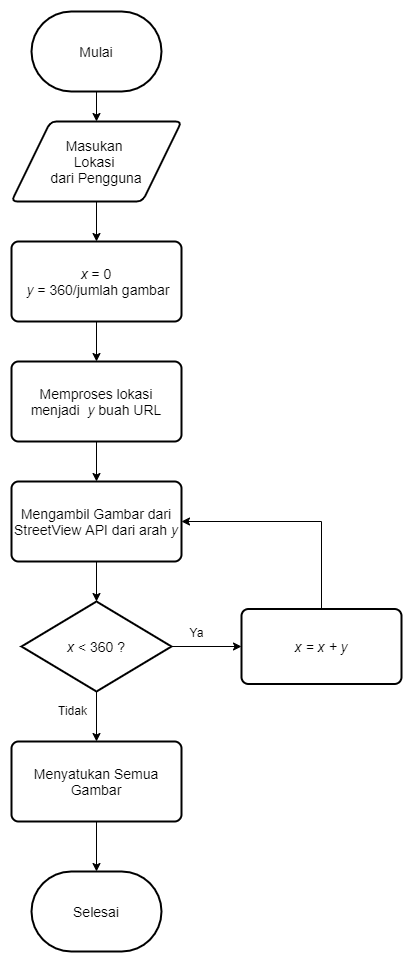
\includegraphics[scale=0.5]{Gambar/streetview-flowchart.png}
	\caption{\textit{Flowchart} dari Proses Memperoleh dan Menyatukan Gambar dari \textit{StreetView API}}
	\label{fig:streetview-flowchart}
\end{figure}

Peubah \textit{i} pada \textit{flowchart} digunakan untuk iterasi semua elemen \textit{array} arrSteps. Untuk setiap iterasi, URL untuk mengakses \textit{StreetView API} dibuat sebanyak jumlah gambar yang ingin dihasilkan. Arah atau \textit{heading} dari gambar-gambar yang dihasilkan ditentukan dengan peubah \textit{x} pada \textit{flowchart}. Peubah \textit{y} merupakan selisih \textit{heading} dari satu iterasi ke iterasi yang berikutnya. Nilai 360 menunjuk pada 360 derajat dalam satu putaran. Untuk mendapatkan pemandangan yang sekeliling yang penuh, gambar dari setiap derajat ke-\textit{x} selama nilai \textit{x} masih bernilai lebih kecil dari 360. Setelah gambar-gambar  itu sudah diperoleh dari \textit{StreetView API}, gambar-gambar tersebut harus disatukan, lalu gambar itu dapat disimpan dalam \textit{file}, lalu gambar dalam \textit{file} itu dapat digunakan.


\subsubsection{Pemanfaatan Sensor \textit{Step Detector}}
Sensor \textit{step detector} digunakan untuk mendeteksi langkah kaki pengguna. Untuk membentuk skenario yang tepat untuk memungkinkan perubahan pemandangan yang sudah ditangani oleh \textit{StreetView} dan \textit{Directions API}, waktu perubahan dari pemandangan itulah yang harus ditangani. Sensor \textit{step detector}lah yang akan menangani bagian waktu perubahan pemandangan. 

Dari \textit{JSON Object} dengan\textit{key "steps"}, dapat diperoleh \textit{JSON Object} dengan \textit{key "distance"} yang memiliki  nilai \textit{"value"}. \textit{"Value"} dari \textit{"distance"} menunjuk pada jarak dari \textit{"step"} yang diacu. Untuk berlari sesuai dengan jarak itu, harus ada sebuah peubah bertipe numerik (\textit{integer}) yang menandakan \textit{progress} perjalanan pelari, lalu harus ada sebuah konstan yang menyatakan jarak dari satu langkah. Peubah yang mencatat \textit{progress} akan bertambah setiap kali sensor mendeteksi langkah kaki. Jika \textit{progress} sudah mencapai nilai jarak dari \textit{step} saat ini, pemandangan VR berulah dapat diubah dengan gambar pemandangan dari \textit{step} berikutnya. Algoritma \ref{alg:algoritma-step-detector} menunjukkan hal-hal yang terjadi saat  sensor \textit{step detector} menerima rangsang. 

\begin{algorithm}
	\caption{Algoritma Saat \textit{Step Detector} Menerima Rangsang}
	\label{alg:algoritma-step-detector}
	\begin{algorithmic}[1]
	\Function{onStepDetectorChanged}{$stepsDist$}
		\State $distanceElapsed \gets 0$ 
		\State $currentStepDist \gets first$ $element$ $of$ $stepsDist.value$ 
		\If{sensor detects footstep}
    		\State $distanceElapsed \gets distanceElapsed + DISTANCE\_PER\_STEP$
    		\If{$distanceElapsed < currentStepDist.value$}
													\If{$currentStepDist.Next IS NOT NULL$}
    			\State $currentStepDist \gets currentStepDist.value + currentStepDist.next$
    		\EndIf
    	\EndIf
    	\EndIf
	\EndFunction  
	\end{algorithmic}
\end{algorithm}

\textit{StepsDist} merupakan \textit{array} dari \textit{steps distance}. \textit{DistanceElapsed} merupakan peubah yang mencatat \textit{progress} langkah dari pengguna, sementara \textit{currentStepDist} merupakan peubah yang mencatat jarak yang harus ditempuh untuk mencapai \textit{steps distance} berikutnya.
Peubhan \textit{distanceElapsed} akan ditambah dengan konstanta \textit{DISTANCE\_PER\_STEP} setiap kali ada langkah kaki yang terdeteksi.
Jika \textit{distanceElapsed} sudah mecapai \textit{curStepDistance}, \textit{curStepDistances} akan ditambah dengan nilai \textit{step distance} selanjutnya. 



